\section{Algoritmo del Banquero}
El Algoritmo del banquero en sistemas operativos es una forma de evitar el
\emph{deadlock}, propuesta por primera vez por Edsger Dijkstra. Es un
acercamiento te'orico para evitar los \emph{deadlocks} en la planificaci'on de
recursos. Requiere conocer con anticipaci'on los recursos que ser'an utilizados
por todos los procesos. Esto 'ultimo generalmente no puede ser satisfecho en la
pr'actica.
El algoritmo mantiene al sistema en un estado seguro. Un sistema se encuentra
en un estado seguro si existe un orden en que pueden concederse las peticiones
de recursos a todos los procesos, previniendo el \emph{deadlock}.
Los procesos piden recursos, y son complacidos siempre y cuando el sistema se
mantenga en un estado seguro despu'es de la concesi'on. De lo contrario, el
proceso es suspendido hasta que otro proceso libere recursos suficientes.
En t'erminos m'as formales, un sistema se encuentra en un estado seguro si
existe una secuencia segura. Una secuencia segura es una sucesi'on de procesos,
$< P_1,\ldots, P_n >$ , donde para un proceso $P_i$, el pedido de recursos
puede ser satisfecho con los recursos disponibles sumados los recursos que
están siendo utilizados por $P_j$, donde $j < i$. Si no hay suficientes
recursos para el proceso $P_i$, debe esperar hasta que alg'un proceso $P_j$
termine su ejecuci'on y libere sus recursos. Reci'en entonces podr'a $P_i$
tomar los recursos necesarios, utilizarlos y terminar su ejecuci'on. Al suceder
esto, el proceso $P_{i+1}$ puede tomar los recursos que necesite, y as'i
sucesivamente. Si una secuencia de este tipo no existe, el sistema se dice que
está en un estado inseguro, aunque esto no implica que esté bloqueado.
Así, el uso de este tipo de algoritmo permite impedir el \emph{deadlock}, pero
supone una serie de restricciones:
\begin{itemize}
 \item Se debe conocer la m'axima demanda de recursos por anticipado.
 \item Los procesos deben ser independientes, es decir que puedan ser
ejecutados en cualquier orden. Por lo tanto su ejecución no debe estar forzada
por condiciones de sincronizaci'on.
 \item Debe haber un número fijo de recursos a utilizar y un número fijo de
procesos.
 \item Los procesos no pueden finalizar mientras retengan recursos.
\end{itemize}
En este trabajo realizamos un simulador para el Algoritmo del Banquero. La idea
principal de este simulador es mostrar paso a paso la ejecuci'on del algoritmo
para una instancia que el usuario provea, asi el usuario podr'a saber si se
trata de un sistema que se encuentra en estado seguro o inseguro.

Mostraremos a continuaci'on el ejercicio 7.c de la guia de ejercicios de la materia. Este ejemplo cuenta con cinco procesos y cuatro recursos.
\begin{figure}
\centering
 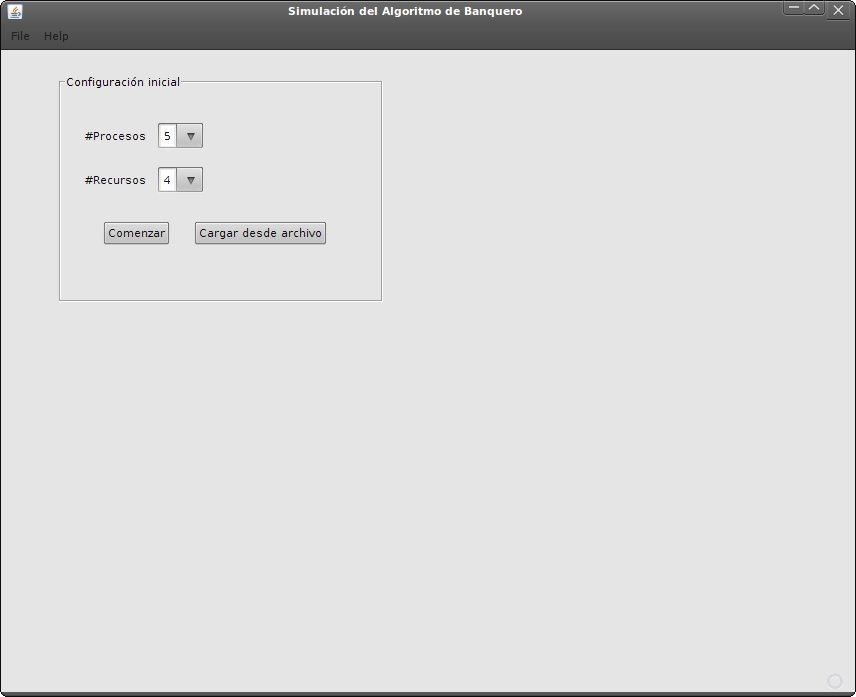
\includegraphics[scale=0.4,keepaspectratio=true]{./imagenes/banquero/banquero1.png}
 \caption{Esta es la primer pantalla del simulador, debemos escoger la cantidad de procesos y recursos o levantar una instancia guardada previamente desde el disco.}
\end{figure}
\begin{figure}
\centering
 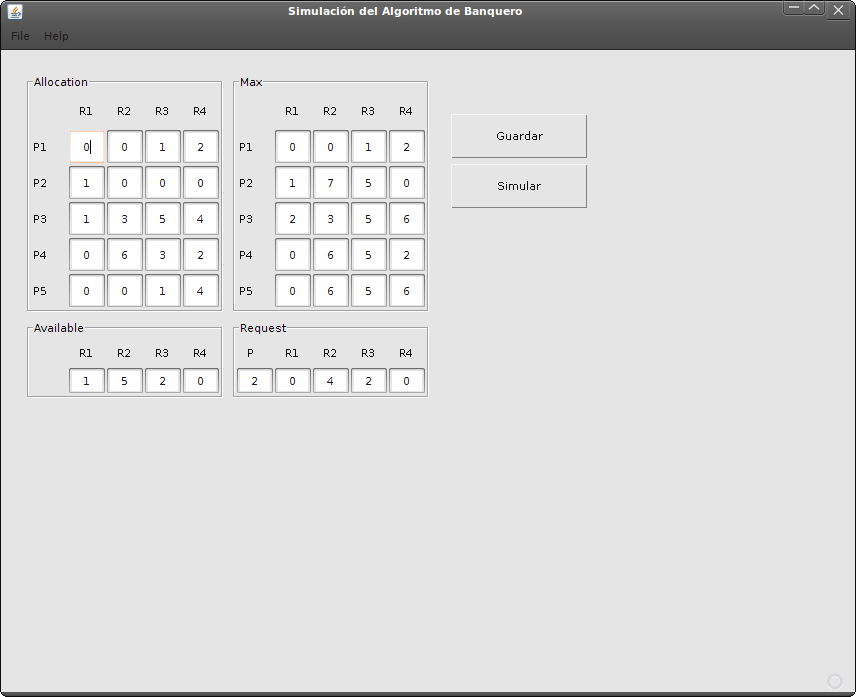
\includegraphics[scale=0.4,keepaspectratio=true]{./imagenes/banquero/banquero2.png}
 \caption{Aqu'i ya vemos la siguiente pantalla, en la que debemos ingresar los valores de entrada de la simulaci'on. \emph{Allocation} es la matriz que refleja los recursos que tiene alocado cada proceso, \emph{Max} es el m'aximo de recursos que un proceso puede usar, \emph{Available} es la cantidad de recursos de cada tipo que no est'an asigandos, \emph{Request} muestra cu'antos recursos de casa tipo pidi'o el proceso \emph{P}. Despu'es de ingresar los valores podemos optar por guardar los valores ingresados para ser usados luego, para esto utilizamos el bot'on \emph{Guardar}.}
\end{figure}
\begin{figure}
\centering
 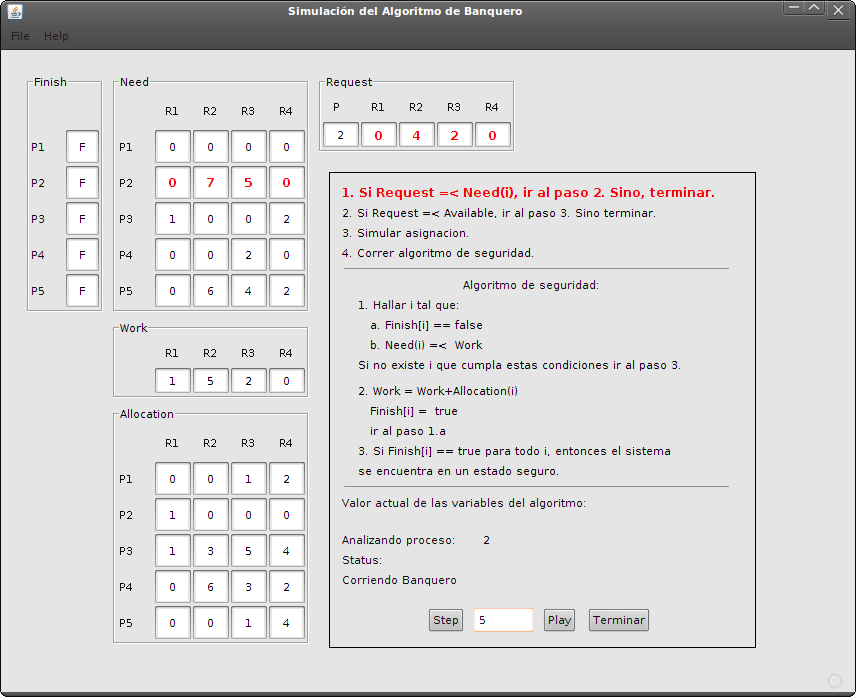
\includegraphics[scale=0.4,keepaspectratio=true]{./imagenes/banquero/banquero3.png}
 \caption{Esta es la 'ultima pantalla del simulador, en ella vemos los valores de las distintas matrices que participan en el algoritmo. El vector \emph{Finish} nos indicar'a cuales de los procesos pueden terminar, si todo el vector \emph{Finish} queda en \emph{True}, querr'a decir que el sistema esta en un estado seguro. El bot'on \emph{Step} avanza el algoritmo un paso, podemos presionarlo repetidas veces hasta finalizar la simulaci'on, tambi'en podemos elegir un intervalo y presionar \emph{Play}. En rojo se mostrar'a el paso del algoritmo que se est'a por ejecutar y los valores que se est'an utilizando en ese paso.} 
\end{figure}
\begin{figure}
\centering
 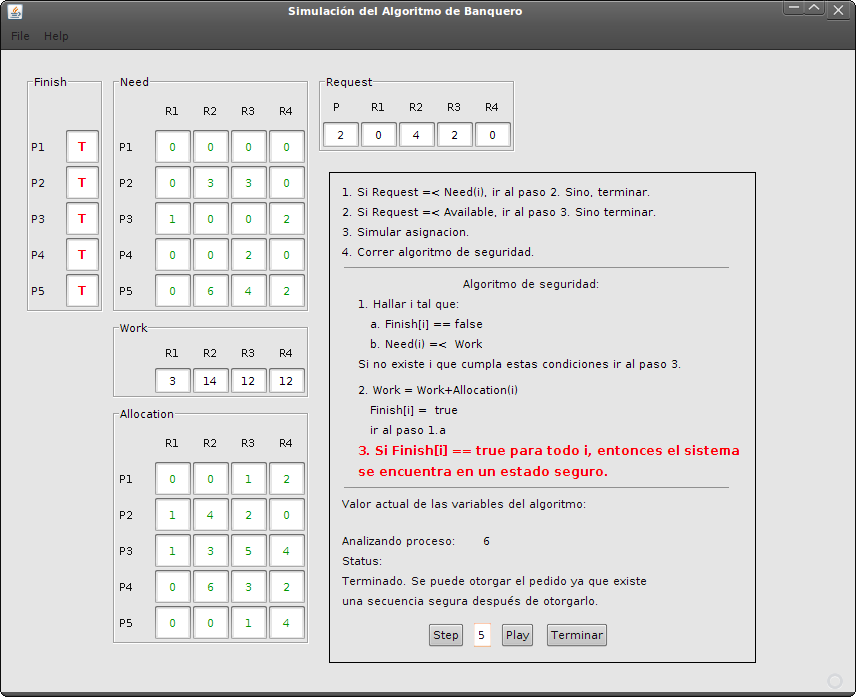
\includegraphics[scale=0.4,keepaspectratio=true]{./imagenes/banquero/banquero4.png}
 \caption{Aqui ya ha terminado la simulaci'on, podemos ver el vector de \emph{Finish} completamente seteado en \emph{True}, eso nos indica que existe una secuencia segura en este sistema.} 
\end{figure}